\documentclass[border=3pt]{standalone}
\usepackage{tikz}
\usetikzlibrary{arrows.meta, positioning, decorations.pathreplacing}
\usetikzlibrary{calc}

\begin{document}

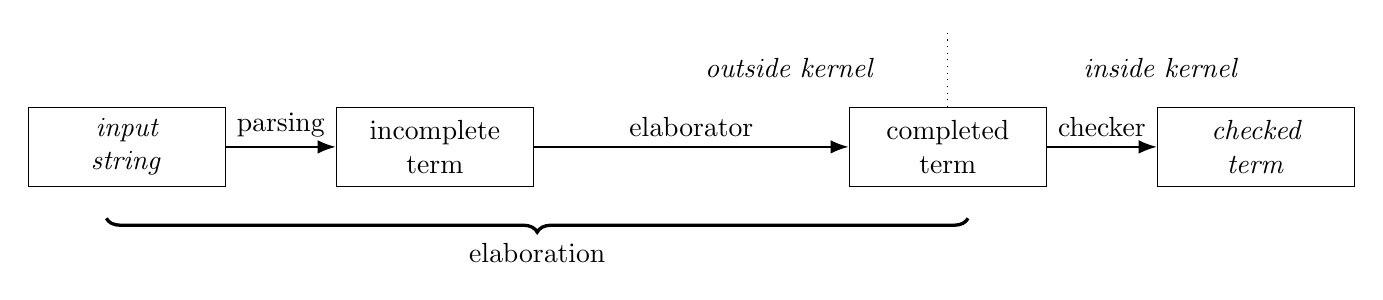
\begin{tikzpicture}[
    box/.style={draw, rectangle, minimum width=2.5cm, minimum height=1cm, align=center},
    arrow/.style={-{Latex}, thick}
]

% Nodes
\node[box, text width=1.5cm] (input) {\textit{input string}};
\node[box, right=1.4cm of input, text width=1.7cm] (incomplete) {incomplete term};
\node[box, right=4cm of incomplete, text width=1.7cm] (completed) {completed term};
\node[box, right=1.4cm of completed, text width=1.3cm] (checked) {\textit{checked term}};

% Arrows
\draw[arrow] (input) -- node[above]{parsing} (incomplete);
\draw[arrow] (incomplete) -- node[above]{elaborator} (completed);
\draw[arrow] (completed) -- node[above]{checker} (checked);

% Outside / inside kernel labels
\node at ($(completed.north) + (-2,.5)$) (outside) {\textit{outside kernel}};
\node at ($(checked.north) + (-1.2,.5)$) (inside) {\textit{inside kernel}};

% Dotted line separating kernels
\draw[dotted] (completed.north) -- ++(0,1cm);

% Braces for elaboration
\draw[decorate, decoration={brace, amplitude=5pt, mirror},line width=1.2pt] 
    ($(input.south west) + (1,-0.4)$) -- ($(completed.south east)+ (-1,-0.4)$) node[midway, below=5pt]{elaboration};

\end{tikzpicture}

\end{document}